\documentclass[dvipdfmx,12pt]{beamer}
\usepackage{bxdpx-beamer}
\usepackage{amsmath}
\usepackage{listings,jlisting}
\usepackage{lstbayes}
\usepackage{minijs}
%\usepackage{helvet}
%\usepackage[helvet]{sfmath}
\usepackage{cmbright}
%\usepackage{iwona}

\renewcommand{\kanjifamilydefault}{\gtdefault}

\lstset{%
  language={R},
  basicstyle={\footnotesize\ttfamily},%
  identifierstyle={},%
  commentstyle={},%
  keywordstyle={},%
  ndkeywordstyle={},%
  stringstyle={},
  frame={},
  breaklines=true,
  columns=[l]{fullflexible},%
  numbers=left,%
  xrightmargin=0zw,%
  xleftmargin=3zw,%
  numberstyle={\scriptsize},%
  stepnumber=1,
  numbersep=1em,%
  lineskip=-0.5ex,%
  keepspaces=true
}

\begin{document}

\title{Stanとdlmによる状態空間モデル\footnote{ファイル一式は\url{https://github.com/ito4303/SappoRoR7}においておきます}}
\author{伊東宏樹}
\date{2016-10-29 SappoRo.R \#7}
\maketitle

%% 状態空間モデル
\begin{frame}{状態空間モデル}
  \begin{center}
    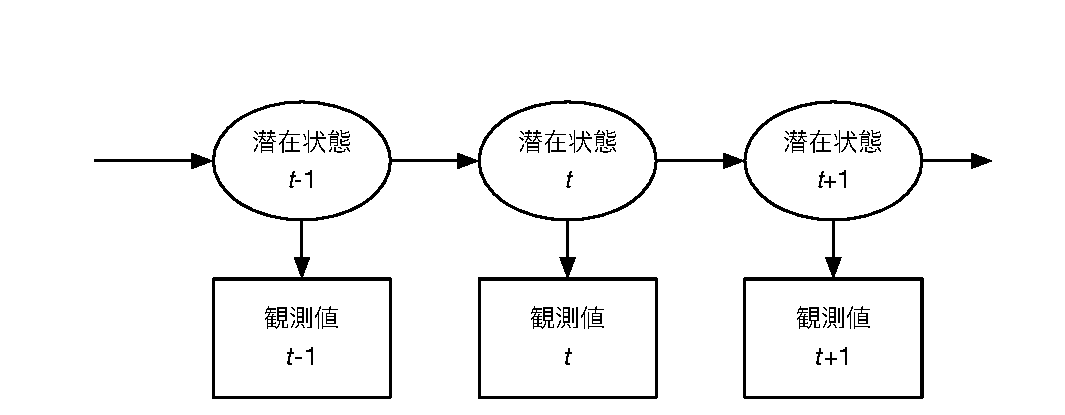
\includegraphics[width=10cm]{ssm}
  \end{center}
\end{frame}

\begin{frame}{状態空間モデル}
  \begin{center}
    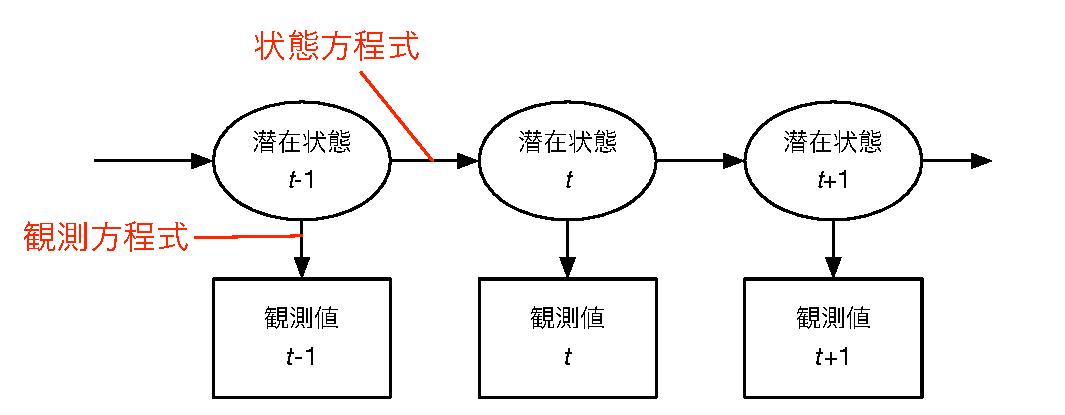
\includegraphics[width=10cm]{ssm2}
  \end{center}
\end{frame}

%% DLM
\begin{frame}{動的線形モデル}
  線形・正規分布の状態空間モデル

  \begin{itemize}
  \item 観測方程式
    \begin{align*}
      \boldsymbol{y}_t &\sim N(\boldsymbol{F}^{\prime} \boldsymbol{\theta}_t, \boldsymbol{V})
    \end{align*}
  \item 状態方程式
    \begin{align*}
      \boldsymbol{\theta}_t &\sim N(\boldsymbol{G} \boldsymbol{\theta}_{t-1}, \boldsymbol{W})
    \end{align*}
  \item 初期値
    \begin{align*}
      \boldsymbol{\theta}_0 &\sim N(\boldsymbol{m}_0, \boldsymbol{C}_0)
    \end{align*}
  \end{itemize}

\end{frame}

%% ローカルレベルモデル
\begin{frame}{ローカルレベルモデル}
  1階差分の動的線形モデル

  \begin{itemize}
  \item 観測方程式
    \begin{align*}
      y_{t} &= \theta_{t} + v_{t}, \quad v_{t} \sim N(0, \sigma_{v}^2) \\
      \downarrow \\
      F &= 1, V = \sigma_{v}^2
    \end{align*}

  \item 状態方程式
    \begin{align*}
      \theta_{t} &= \theta_{t-1} + w_{t}, \quad w_{t} \sim N(0, \sigma_{w}^2) \\
      \downarrow \\
      G &= 1, W = \sigma_{w}^2
    \end{align*}
  \end{itemize}
\end{frame}

%% Stan
\begin{frame}{Stan}
  \begin{itemize}
  \item 観測方程式と状態方程式をそのまま\textsf{Stan}コードにすれば、状態の推定ができる
    \begin{itemize}
    \item 『岩波データサイエンスVol.1』や『StanとRでベイズ統計モデリング』の松浦さんのコードを参照
    \end{itemize}
  \item 今回はあえて、\textsf{Stan}の\texttt{gaussian\_dlm\_obs()}分布と、\textsf{R}の\textsf{dlm}パッケージを使ってみる
  \end{itemize}
\end{frame}

%% gaussian_dlm_obs()
\begin{frame}{gaussian\_dlm\_obs}

  \textit{y}~\textasciitilde~\textbf{gaussian\_dlm\_obs}(\textit{F, G, V, W, m0, C0});

  \begin{itemize}
  \item カルマンフィルタのパラメータ(分散)を推定する
  \item 引数は\textsf{dlm}パッケージに対応
  \end{itemize}
\end{frame}

%% カルマンフィルター
\begin{frame}{カルマンフィルター}
  \begin{itemize}
  \item 行列計算により、フィルタリング・平滑化・予測をおこなう
     \begin{description}
     \item[フィルタリング] $\{y_1,y_2,\dots,y_t\}$から$\theta_t$を推定
     \item[平滑化] $\{y_1,y_2,\dots,y_t\}$から$\{\theta_1,\theta_2,\dots,\theta_t\}$を推定
     \item[予測] $\{y_1,y_2,\dots,y_t\}$から$\{\theta_{t+1},\theta_{t+2},\dots\}$および$\{y_{t+1},y_{t+2},\dots\}$を推定
     \end{description}
  \item パラメータとして、観測方程式・状態方程式の共分散行列(と初期値)が必要
  \end{itemize}
\end{frame}

%% dlm
\begin{frame}{dlmパッケージ}
  \begin{itemize}
  \item 動的線形モデル(Dynamic Linear Model)を扱うパッケージ
  \item カルマンフィルター
  \item パラメータの最尤推定
  \item パラメータのベイズ推定
  \end{itemize}
\end{frame}

%% データ
\begin{frame}[fragile]{データ}
  \begin{lstlisting}[language=R]
## ナイル川の流量データ
data(Nile)
  \end{lstlisting}

  \begin{center}
    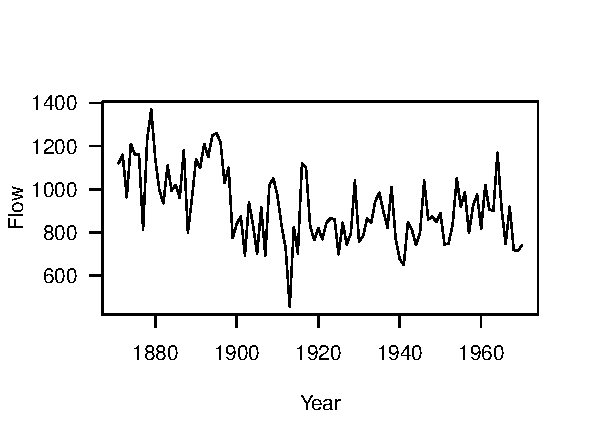
\includegraphics[width=10cm]{Nile}
  \end{center}
\end{frame}

%% ローカルレベルモデルのStanコード
\begin{frame}[fragile]{Stanコード: dataブロック}
  \begin{lstlisting}[language=Stan]
data {
  int<lower=0>  N;   // レコードの数
  matrix[1, N]  Y;   // データ
  real          M0;  // 状態の初期値
  cov_matrix[1] C0;  // 共分散の初期値
}
  \end{lstlisting}
\end{frame}

\begin{frame}[fragile]{Stanコード: transformed dataブロック}
  \begin{lstlisting}[language=Stan]
transformed data {
  matrix[1, 1]  F;
  matrix[1, 1]  G;
  vector[1]     m0; // サイズ1のベクトル

  F[1, 1] = 1;
  G[1, 1] = 1;
  m0[1] = M0;
}
  \end{lstlisting}
\end{frame}

\begin{frame}[fragile]{Stanコード: parametersブロックとtransformed parametersブロック}
  \begin{lstlisting}[language=Stan]
parameters {
  real<lower=0> s2[2];
}

transformed parameters {
  vector[1]     v;
  cov_matrix[1] w;

  v[1] = s2[1];
  w[1, 1] = s2[2];
}
  \end{lstlisting}
\end{frame}

\begin{frame}[fragile]{Stanコード: modelブロック}
  \begin{lstlisting}[language=Stan]
model {
  y ~ gaussian_dlm_obs(F, G, v, w, m0, C0);
}
  \end{lstlisting}
\end{frame}

%% Rから実行
\begin{frame}[fragile]{Rコード}
  \begin{lstlisting}[language=R]
## Stanにわたすデータのリスト
stan_data <- list(N = length(Nile),
                  Y = matrix(Nile, 1),
                  M0 = 100,
                  C0 = matrix(100, 1, 1))

## あてはめ
fit <- stan("dlm1.stan", data = stan_data,
            pars = c("s2"), seed = 1,
            iter = 2000, warmup = 1000)
  \end{lstlisting}
\end{frame}

%% 平滑化
\begin{frame}[fragile]{平滑化}
  \begin{lstlisting}[language=R]
## パラメータの事後平均をとりだす
s2 <- get_posterior_mean(fit, pars = "s2")[, "mean-all chains"]

## Stanで推定したパラメータで、dlmのモデル定義
mod <- dlmModPoly(order = 1,
                  dV = s2[1], dW = s2[2])

## 平滑化
smo <- dlmSmooth(Nile, mod)
  \end{lstlisting}
\end{frame}

%% 平滑化グラフ
\begin{frame}{平滑化}
  \begin{center}
    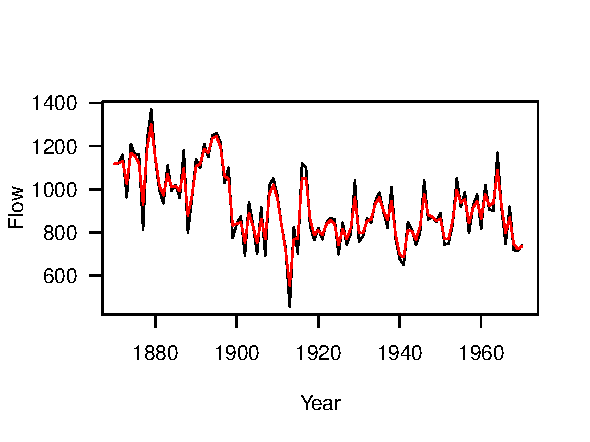
\includegraphics[width=10cm]{dlm1_smooth}
  \end{center}

  赤線が平滑化した値
\end{frame}

%% 予測
\begin{frame}{予測}
  \begin{center}
    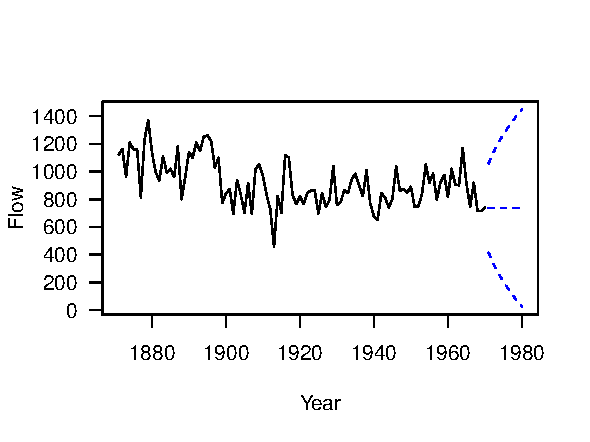
\includegraphics[width=10cm]{dlm1_predict}
  \end{center}

  青実線が予測値, 青点線は80\%予測区間
\end{frame}



%%
%% トレンドモデル
%%
\begin{frame}{トレンドモデル}
  傾きを組み込んだモデル、あるいは2階差分の動的線形モデル

  \begin{itemize}
  \item 観測方程式
    \begin{align*}
      y_{t} &= \theta_{1,t} + v_{t} \\
      \downarrow \\
      y_{t} &= \left(\begin{array}{cc}1 & 0\end{array}\right)
        \left(\begin{array}{c}\theta_{1,t} \\ \theta_{2,t} \end{array}\right) + v_{t} \\
        \downarrow \\
        \boldsymbol{F} &= \left(\begin{array}{c}1 \\ 0\end{array}\right),
          V = \sigma_{v}^2 
    \end{align*}
  \end{itemize}
\end{frame}

\begin{frame}{トレンドモデル}
  \begin{itemize}
  \item 状態方程式
    \begin{align*}
      \theta_{1,t} &= \theta_{1,t-1} + \theta_{2,t-1} + w_{1,t} \\
      \theta_{2,t} &= \theta_{2,t-1} + w_{2,t} \\
      \downarrow \\
      \left(\begin{array}{c}\theta_{1,t} \\ \theta_{2,t}\end{array}\right) &=
      \left(\begin{array}{cc}1 & 1 \\ 0 & 1 \end{array}\right)
      \left(\begin{array}{c}\theta_{1,t-1} \\ \theta_{2,t-1}\end{array}\right) +
      \left(\begin{array}{c}w_{1,t} \\ w_{2,t}\end{array}\right) \\
      \downarrow \\
      \boldsymbol{G} &= \left(\begin{array}{cc}1 & 1 \\ 0 & 1 \end{array}\right),
      \boldsymbol{W} = \left(\begin{array}{cc}\sigma_{w1}^2 & 0\\ 0 & \sigma_{w2}^2\end{array}\right)
    \end{align*}
  \end{itemize}
\end{frame}


%% Stanコード
\begin{frame}[fragile]{dataブロック}
  \begin{lstlisting}[language=Stan]
data {
  int<lower=0>  N;  // レコードの数
  matrix[1, N]  Y;  // データ
  vector[2]     M0;
  cov_matrix[2] C0;
}
  \end{lstlisting}
\end{frame}

\begin{frame}[fragile]{transformed dataブロック}
  \begin{lstlisting}[language=Stan]
transformed data {
  matrix[2, 1]  F;
  matrix[2, 2]  G;

  // F
  F[1, 1] = 1;
  F[2, 1] = 0;

  // G
  G[1, 1] = 1;
  G[1, 2] = 1;
  G[2, 1] = 0;
  G[2, 2] = 1;
}
  \end{lstlisting}
\end{frame}

\begin{frame}[fragile]{parametersブロックとtransformed parametersブロック}
  \begin{lstlisting}[language=Stan]
parameters {
  real<lower=0> s2[3];
}

transformed parameters {
  vector[1]     v;
  cov_matrix[2] w;

  v[1] = s2[1];
  w[1, 1] = s2[2];
  w[1, 2] = 0;
  w[2, 1] = 0;
  w[2, 2] = s2[3];
}
  \end{lstlisting}
\end{frame}

\begin{frame}[fragile]{modelブロック}
  \begin{lstlisting}[language=Stan]
model {
  y ~ gaussian_dlm_obs(F, G, v, w, M0, C0);
}
  \end{lstlisting}
\end{frame}

%% Rコード
\begin{frame}[fragile]{Rコード}
  \begin{lstlisting}[language=R]
## Stanにわたすデータのリスト
stan_data <- list(N = length(Nile),
                  Y = matrix(Nile, 1),
                  M0 = c(100, 1),
                  C0 = matrix(c(1e7, 0, 0, 1e7), 2, 2))

## あてはめ
fit <- stan("dlm2.stan", data = stan_data,
            pars = c("s2"), seed = 1,
            iter = 2000, warmup = 1000)
  \end{lstlisting}
\end{frame}

\begin{frame}[fragile]{Rコード}
  \begin{lstlisting}[language=R]
## パラメータの事後平均をとりだす
s2 <- get_posterior_mean(fit, pars = "s2")[, "mean-all chains"]

## dlmでのモデル定義
mod <- dlmModPoly(order = 2,
                  dV = s2[1], dW = s2[2:3])

## 平滑化
smo <- dlmSmooth(Nile, mod)
  \end{lstlisting}
\end{frame}

\begin{frame}[fragile]{Rコード}
  \begin{lstlisting}[language=R]
## カルマンフィルター
filt <- dlmFilter(Nile, mod)

## 状態
m <- filt$m[-1, ]

## 予測
## 予測する年数
nyear <- 10

## 予測期間の初期値の設定
m0(mod) <- m[length(Nile), ]
C0(mod) <- diag(2) * s2[2:3]

fore <- dlmForecast(mod, nAhead = nyear)
  \end{lstlisting}
\end{frame}

%% 平滑化グラフ
\begin{frame}{平滑化}
  \begin{center}
    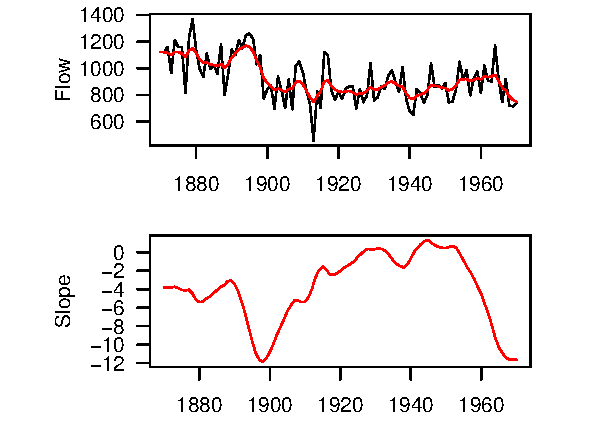
\includegraphics[width=10cm]{dlm2_smooth}
  \end{center}

  赤線が平滑化した値
\end{frame}

%% 予測
\begin{frame}{予測}
  \begin{center}
    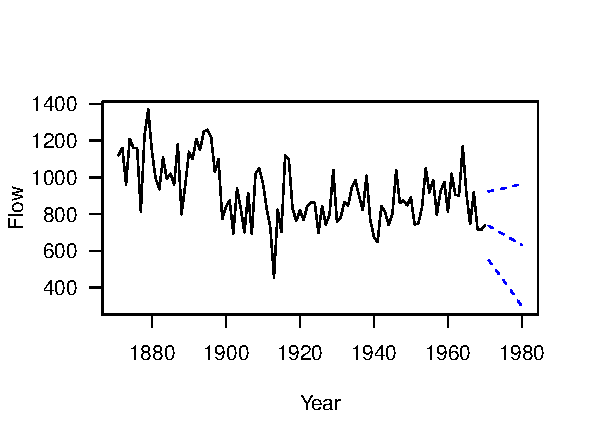
\includegraphics[width=10cm]{dlm2_predict}
  \end{center}

  青実線が予測値, 青点線は80\%予測区間
\end{frame}

%% まとめ
\begin{frame}{まとめ}
  \begin{itemize}
  \item \textsf{Stan}の\texttt{gaussian\_dlm\_obs}分布で動的線形モデルの
    パラメータを推定することができる。
  \item 推定したパラメータの値を\textsf{dlm}パッケージの関数で使用して
    カルマンフィルタを適用できる。
  \end{itemize}
\end{frame}

\begin{frame}{まとめ}
  \begin{itemize}
  \item とはいえ、普通に状態をベイズ推定するなら、全部\textsf{Stanで}モデルを
    書くほうがてっとりばやいかも。

  \end{itemize}
\end{frame}

\end{document}
